\todo[inline]{Add use case coverage of requirements}
\section{Use case scenarios}
Now we are going to depict goals of users which the application will make achievable.
Figure 2.1 contains a use case diagram of the application.
A use case styled with a bold border groups together more use cases and will be further expanded.
All use cases will be structurally described by independent use case scenarios.
A scenario will contain its description only if the goal of a user is not clear from a use case's name.

\todo[inline]{Update name of a use case Warn my guests...}

\begin{figure}[h]
  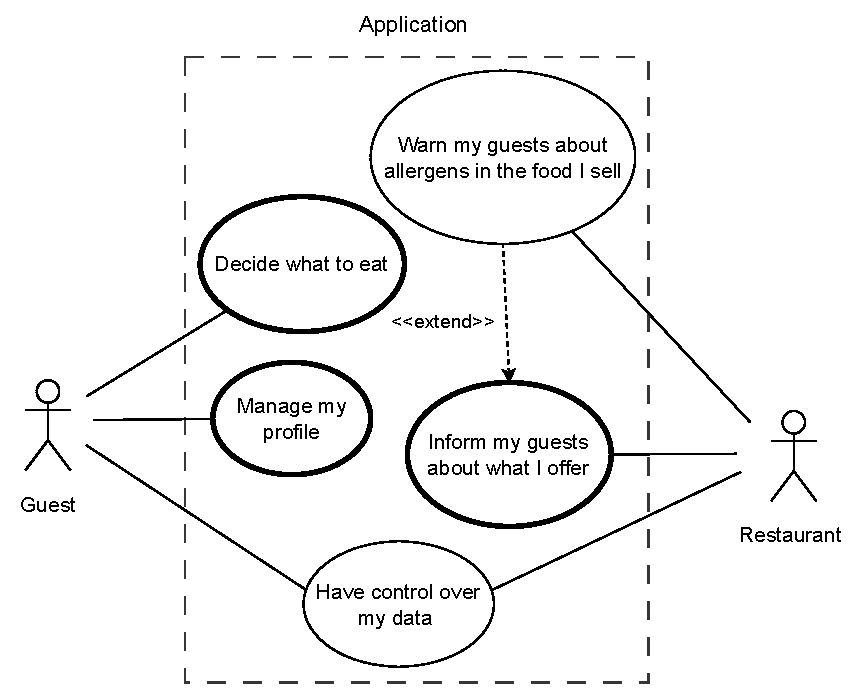
\includegraphics[width=\linewidth]{master-thesis/img/use-cases/use_cases}
  \caption{The application's use case diagram.}
\end{figure}

\newpage

% Add top padding for scenario tables
\def\arraystretch{1.5}

\subsection{Guest use cases}

\todo[inline]{change ids of use cases}
\textbf{UC1: Find a meal I can eat at a restaurant}
\begin{center}
  \begin{tabular}{| l | p{10.75cm} | }
    \hline
    Actor        & Guest \\
    \hline
    Description  & A guest comes to a restaurant and is deciding what to order. \\
    \hline
    Precondition & The guest has created a profile. \\
    \hline
    Postcondition & The guest sees only the items of the menu which they can eat. \\
    \hline
    Scenario     &
    \begin{minipage}[t]{\linewidth}
      \begin{enumerate}[leftmargin=*,nosep,before=\vspace{-0.575\baselineskip},after=\strut]
        \item The guest scans a QR code on a printed menu which takes them to the application.
        \item The application displays a personalized menu based on the guest's profile. \textbf{A1}
      \end{enumerate}
    \end{minipage}
    \\
    \hline
    Alternatives &
    \begin{minipage}[t]{\linewidth}
      \begin{description}[nosep,after=\strut]
        \item [A1:] The guest selects that they wish to see the full menu by clicking the button labeled as "Display full menu". The application shows a warning which says that the menu may contain food items which the guest is allergic to. The guest reads the warning and decides to proceed. The application displays a menu with no personalization.
      \end{description}
    \end{minipage}
    \\
    \hline
  \end{tabular}
  \newline
\end{center}

\begin{figure}[h]
  \centering
  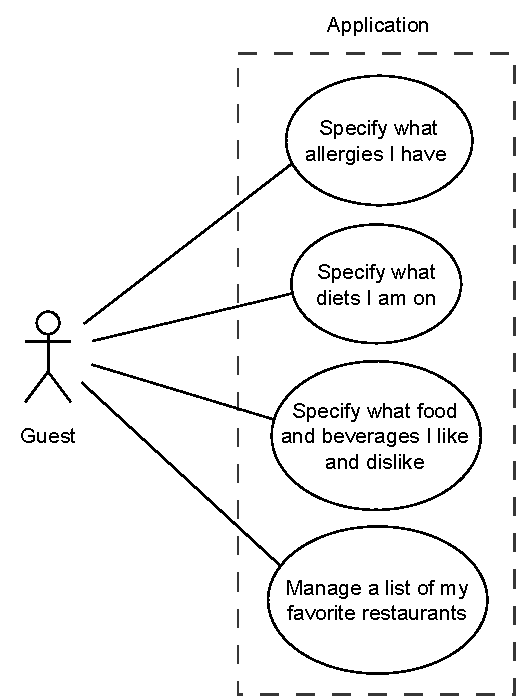
\includegraphics[width=0.62\linewidth]{master-thesis/img/use-cases/use_cases_guest_profile_management}
  \caption{Guest profile management use cases}
\end{figure}

\newpage

\noindent \textbf{UC2: Use case: Specify what allergies I have}
\begin{center}
  \begin{tabular}{| l | p{10.75cm} | }
    \hline
    Actor       & Guest \\
    \hline
    Scenario    &
    \begin{minipage}[t]{\linewidth}
      \begin{enumerate}[leftmargin=*,nosep,before=\vspace{-0.575\baselineskip},after=\strut]
        \item The guest opens their profile and navigates to a section for managing allergies.
        \item The application displays a screen with a list of previously specified allergies by the guest. \textbf{A1}
        \item The guest presses a button labeled as "Add allergy".
        \item The application displays a search bar.
        \item The guest starts typing the name of an allergy into the search bar.
        \item The application suggests allergies which contain the given input in their name.
        \item The guest selects the desired allergy and presses an "Add" button. \textbf{A2}
        \item The application adds the specified allergy the guest's profile. \textbf{A3}
        \item The guest repeats steps 3 to 8 until they have specified all of the food allergies they suffer from.
      \end{enumerate}
    \end{minipage}
    \\
    \hline
    Alternatives &
    \begin{minipage}[t]{\linewidth}
      \begin{description}[nosep,after=\strut]
        \item [A1:] The list is empty because the guest has not specified any allergies yet. The application displays a text containing this information.
        \item [A2:] The application does not recognize the allergy which the guest is trying to specify. The guest creates a public issue in the application's repository with a request to add the desired allergy to the application.
        \item [A3:] The allergy the guest has specified is already contained in the guest's profile. The application informs the guest about this fact and their profile is not altered.
      \end{description}
    \end{minipage}
    \\
    \hline
  \end{tabular}
  \newline
\end{center}

\noindent \textbf{UC3: Look up online what a restaurant offers today}
\begin{center}
  \begin{tabular}{| l | p{10.75cm} | }
    \hline
    Actor        & Guest \\
    \hline
    Description  & A guest is at home or on their way to a restaurant and wants to know what the restaurant serves at the moment. \\
    \hline
    Scenario     &
    \begin{minipage}[t]{\linewidth}
      \begin{enumerate}[leftmargin=*,nosep,before=\vspace{-0.575\baselineskip},after=\strut]
        \item The guest visits the restaurant's webpage and clicks on a link which takes them to the application. \textbf{A1 A2}
        \item The application displays a menu.           
      \end{enumerate}
    \end{minipage}
    \\
    \hline
    Alternatives &
    \begin{minipage}[t]{\linewidth}
      \begin{description}[nosep,after=\strut] 
        \item [A1:] The guest selects a restaurant in the overview screen from UC4. The application lists all menus of the chosen restaurant. The guest selects one of the menus. The application displays the menu.
        \item [A2:] The guest specifies the IRI of the restaurant. The application lists all menus of the chosen restaurant. The guest selects one of the menus. The application displays the menu.
      \end{description}
    \end{minipage}
    \\
    \hline
  \end{tabular}
  \newline
\end{center}

\newpage

\todo[inline]{Make the figure bigger - increase height, make bubbles bigger}

\begin{figure}[h]
  \centering
  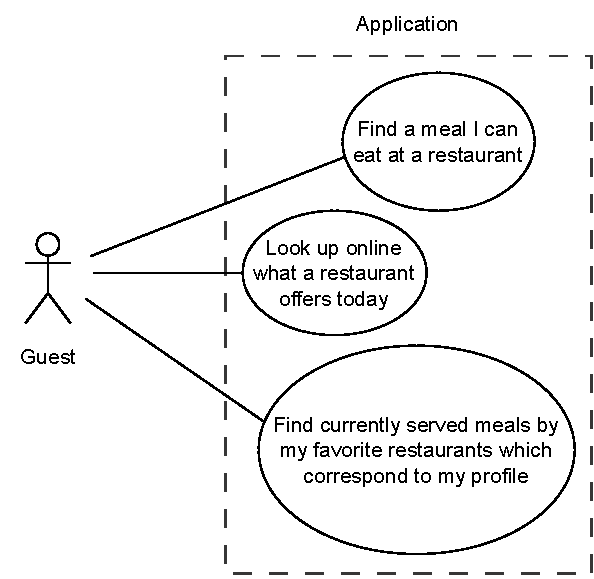
\includegraphics[width=0.62\linewidth]{master-thesis/img/use-cases/use_cases_guest_menu_viewer}
  \caption{Guest menu viewing use cases}
\end{figure}

\todo[inline]{change name (also in figure) to "Find currently served meals by my favorite restaurants which I can eat"}
\noindent \textbf{UC4: Find currently served meals by my favorite restaurants which correspond to my profile}
\begin{center}
  \begin{tabular}{| l | p{10.75cm} | }
    \hline
    Actor        & Guest \\
    \hline
    Description  & A guest wants to know what do their favorite restaurants currently have to offer. \\
    \hline
    Precondition & The guest is logged in to the application. \\
    \hline
    Postcondition & The guest sees a list of their favorite restaurants with selected items from their menus. \\
    \hline
    Scenario     &
    \begin{minipage}[t]{\linewidth}
      \begin{enumerate}[leftmargin=*,nosep,before=\vspace{-0.575\baselineskip},after=\strut]
        \item The application displays an overview of what the guest's favorite restaurants currently serve. \textbf{A1}\textbf{A2} \textbf{A3}
      \end{enumerate}
    \end{minipage}
    \\
    \hline
    Alternatives &
    \begin{minipage}[t]{\linewidth}
      \begin{description}[nosep,after=\strut]
        \item [A1:] The restaurants do not currently serve anything. The application displays a text with this information.
        \item [A2:] The overview is empty because the guest has not added any of their favorite restaurants yet. The application displays instructions on how to add a restaurant to the list.
        \item [A2:] A restaurant has no valid menu published at the moment. The application displays a text with this information close to the restaurant's name.
      \end{description}
    \end{minipage}
    \\
    \hline
  \end{tabular}
  \newline
\end{center}

\newpage

\noindent \textbf{5. Use case: Specify what diets I am on}
\begin{center}
  \begin{tabular}{| l | p{10.75cm} | }
    \hline
    Actor       & Guest \\
    \hline
    Scenario    &
    \begin{minipage}[t]{\linewidth}
      \begin{enumerate}[leftmargin=*,nosep,before=\vspace{-0.575\baselineskip},after=\strut]
        \item The guest opens their profile and navigates to a section for managing diets.
        \item The application displays a screen with a list of previously specified diets by the guest. \textbf{A1}
        \item The guest presses a button labeled as "Add diet".
        \item The application displays a search bar.
        \item The guest starts typing the name of a diet into the search bar.
        \item The application suggests diets which contain the given input in their name.
        \item The guest selects the desired diet and presses an "Add" button. \textbf{A2}
        \item The application adds the specified diet to the guest's profile. \textbf{A3}
        \item The guest repeats steps 3 to 8 until they have specified all of the diets they are on.
      \end{enumerate}
    \end{minipage}
    \\
    \hline
    Alternatives &
    \begin{minipage}[t]{\linewidth}
      \begin{description}[nosep,after=\strut]
        \item [A1:] The list is empty because the guest has not specified any diets yet. The application displays a text containing this information.
        \item [A2:] The application does not recognize the diet which the guest is trying to specify. The guest creates a public issue in the application's repository with a request to add the desired diet to the application.
        \item [A3:] The diet the guest has specified is already contained in the guest's profile. The application informs the guest about this fact and their profile is not altered.
      \end{description}
    \end{minipage}
    \\
    \hline
  \end{tabular}
  \newline
\end{center}

\noindent \textbf{6. Use case: Have control over my data}
\begin{center}
  \begin{tabular}{| l | p{10.75cm} | }
    \hline
    Actor        & Guest \\
    \hline
    Description  & A guest wants to specify where should the application store and read their data. \\
    \hline
    Scenario     &
    \begin{minipage}[t]{\linewidth}
      \begin{enumerate}[leftmargin=*,nosep,before=\vspace{-0.575\baselineskip},after=\strut]
        \item The guest navigates to a page for managing data storage options.
        \item The application provides a list of places where it can store data.
        \item The guest selects one of the options.
        \item The application starts using the selected place for storing and reading the guest's data.
      \end{enumerate}
    \end{minipage}
    \\
    \hline
  \end{tabular}
  \newline
\end{center}

\newpage

\noindent \textbf{7. Use case: Specify what food and beverages I like and dislike}
\begin{center}
  \begin{tabular}{| l | p{10.75cm} | }
    \hline
    Actor    & Guest \\
    \hline
    Scenario &
    \begin{minipage}[t]{\linewidth}
      \begin{enumerate}[leftmargin=*,nosep,before=\vspace{-0.575\baselineskip},after=\strut]
        \item The guest opens their profile and navigates to a section for managing food preferences.
        \item The application displays a screen with two lists, one containing the foods which the guest likes and the other containing the foods which the guest dislikes. \textbf{A1}
        \item The guest presses a button labeled as "Add food" at the end of the list of foods which they like. \textbf{A2}
        \item The application displays a search bar.
        \item The guest starts typing the name of a food into the search bar.
        \item The application suggests foods which contain the given input text in their name.
        \item The guest selects the desired food and presses an "Add" button. \textbf{A3}
        \item The application adds the specified food to the guest's profile. \textbf{A4}
        \item The guest repeats steps 3 to 8 until they have specified all of their food preferences.
      \end{enumerate}
    \end{minipage}
    \\
    \hline
    Alternatives &
    \begin{minipage}[t]{\linewidth}
      \begin{description}[nosep,after=\strut]
        \item [A1:] Either one or both of the lists are empty because the guest has not specified any of their preferences yet. The application displays a text which informs the guest about this fact.
        \item [A2:] The guest presses a button labeled as "Add food" at the end of the list of foods which they dislike.
        \item [A3:] The application does not recognize the food which the guest is trying to specify. The guest creates a public issue in the application's repository with a request to add the desired food to the application.
        \item [A4:] The guest's profile already contains the specified food. The guest is informed about this fact and their profile is not altered.
      \end{description}
    \end{minipage}
    \\
    \hline
  \end{tabular}
  \newline
\end{center}

\newpage

\noindent \textbf{8. Use case: Manage a list of my favorite restaurants}
\begin{center}
  \begin{tabular}{| l | p{10.75cm} | }
    \hline
    Actor    & Guest \\
    \hline
    Scenario &
    \begin{minipage}[t]{\linewidth}
      \begin{enumerate}[leftmargin=*,nosep,before=\vspace{-0.575\baselineskip},after=\strut]
        \item The guest opens their profile and navigates to a section where they can manage their favorite restaurants. \textbf{A1}
        \item The application displays a screen with a list containing the guest's favorite restaurants. \textbf{A2} 
        \item The guest presses a button for adding a restaurant to~the~list.~\textbf{A3}
        \item The application provides a text input field. 
        \item The guest specifies the IRI of a restaurant which they wish to add to the list and presses an "Add" button. 
        \item The application adds the restaurant to the~guest's~profile.~\textbf{A4}~\textbf{A5}
      \end{enumerate}
    \end{minipage}
    \\
    \hline
    Alternatives &
    \begin{minipage}[t]{\linewidth}
      \begin{description}[nosep,after=\strut]
        \item [A1:] The guest is viewing a restaurant's detail. The guest presses a button for marking the restaurant as their favorite. The application adds the restaurant to the guest's profile. \textbf{A1.b}
        \item [A1.b:] The restaurant is already contained in the guest's profile and pressing the button removes the restaurant from it.
        \item [A2:] The list is empty because the guest has not added any restaurants yet. The application displays a text containing this information.
        \item [A3:] The guest presses a button for removing a restaurant. The application removes the restaurant from the guest's profile.
        \item [A4:] The guest's profile already contains the restaurant by the specified IRI. The guest is informed about this fact and their profile is not altered.
        \item [A5:] The IRI which the guest specified is not valid. The application informs the guest about this fact and the scenario continues with step 3.
      \end{description}
    \end{minipage}
    \\
    \hline
  \end{tabular}
  \newline
\end{center}

\newpage
